\documentclass[12pt]{amsart}

\usepackage[margin=1in]{geometry}

\usepackage{amsmath,amssymb,amsthm}
\usepackage{hyperref}
\usepackage{tikz,tikz-cd}
\usetikzlibrary{calc}
\usepackage{xcolor}

\newtheorem{theorem}{Theorem}
\newtheorem{lemma}[theorem]{Lemma}
\newtheorem{proposition}[theorem]{Proposition}
\newtheorem{corollary}[theorem]{Corollary}
\newtheorem{conjecture}[theorem]{Conjecture}
\theoremstyle{definition} \newtheorem*{notation}{Notation}
\theoremstyle{remark} \newtheorem*{remark}{Remark}
\theoremstyle{remark} \newtheorem*{example}{Example}
\theoremstyle{definition} \newtheorem*{definition}{Definition}

\numberwithin{equation}{section}
\numberwithin{theorem}{section}

\renewcommand{\pmod}[1]{\left(\mathrm{mod}\,#1\right)}

\title{Arithmetic statistics course notes}

\author{Robert J. Lemke Oliver}
\date{\today}

\begin{document}

	\maketitle
	
	\setcounter{section}{1}
	
\section{Rings of integers and discriminants}
	
	We now turn to considering what will prove to be some of the most fundamental objects to this course, namely \emph{rings of integers}.  We begin with several definitions and lemmas.
	
	\subsection{Algebraic integers}
	
	\begin{definition}
		A number $\alpha \in \mathbb{C}$ is called an \emph{algebraic integer} if it is the root of a monic polynomial $f \in \mathbb{Z}[x]$.
	\end{definition}
	
	We've given this definition relative to roots of any monic integer polynomial because that's the definition that's easiest to check, but in fact, we could have defined it relative to irreducible polynomials only (as are usually considered when dealing with field extensions).
	
	\begin{lemma}
		A number $\alpha$ is an algebraic integer if and only if it is the root of an irreducible monic polynomial $f \in \mathbb{Z}[x]$.
	\end{lemma}
	\begin{proof}
		One direction is immediate: if $\alpha$ is the root of an irreducible monic polynomial, then it's an algebraic integer by definition.
		
		Conversely, suppose that $\alpha$ is the root of some monic integer polynomial, $f \in \mathbb{Z}[x]$.  If $f$ is not irreducible, then it must factor as $f = f_1 f_2$.  We thus find $f(\alpha) = f_1(\alpha) f_2(\alpha)$, but $f(\alpha)=0$, so either $f_1(\alpha)=0$ or $f_2(\alpha)=0$ since $\mathbb{C}$ is a field; suppose $f_1(\alpha)=0$.  If $f_1$ is irreducible, we're done, and if not, we can repeat this process, eventually ending at an irreducible polynomial of which $\alpha$ is a root.
	\end{proof}
	
	We next show that the set of all algebraic integers forms a ring under the conventional notions of addition and multiplication.  This is provided by the following lemma.
	
	\begin{lemma}\label{lem:integers-closed}
		Suppose $\alpha$ and $\beta$ are algebraic integers.  Then both $\alpha+\beta$ and $\alpha \beta$ are algebraic integers as well.
	\end{lemma}
	\begin{proof}[Proof sketch]
		We begin with some preliminary observations.  By definition, both $\alpha$ and $\beta$ are roots of monic integer polynomials, say
			\[
				f_\alpha(x) = x^n + a_1 x^{n-1} + \dots + a_n, \quad f_\beta(x) = x^m + b_1 x^{m-1} + \dots + b_m.
			\]
		We will find it useful to aslso factor $f_\alpha$ and $f_\beta$ over $\mathbb{C}$.  By the fundamental theorem of algebra, they each factor completely into linear polynomials, say
			\[
				f_\alpha(x) = \prod_{i=1}^n (x-\alpha_i), \quad f_\beta(x) = \prod_{j=1}^m (x-\beta_j).
			\]
		Necessarily, $\alpha = \alpha_i$ for some $i$, and $\beta = \beta_j$ for some $j$.\footnote{Without loss of generality, you may assume $\alpha = \alpha_1$ and $\beta = \beta_1$, but in fact, the proof we will write down is ``index agnostic,'' and this won't substantially simplify things.}  Observe finally that the coefficients of $f_\alpha$ and $f_\beta$ may therefore be expressed in terms of the roots, e.g.
			\[
				a_1 = -(\alpha_1 + \dots + \alpha_n), \quad a_2 = \alpha_1\alpha_2 + \alpha_1\alpha_3 + \dots + \alpha_{n-1} \alpha_n = \sum_{i_1 < i_2} \alpha_{i_1}\alpha_{i_2},
			\]
		and in general
			\[
				a_k = (-1)^k \sum_{i_1 < i_2 < \dots < i_k} \alpha_{i_1}\alpha_{i_2} \dots \alpha_{i_k},
			\]
		with analogous expressions for the $b_j$.
			
		We now show that $\alpha+\beta$ is an algebraic integer.  Consider the polynomial
			\[
				f_{\alpha+\beta}(x) := \prod_{i=1}^n \prod_{j=1}^m (x-\alpha_i-\beta_j).
			\]
		We claim that, using the expressions for $a_i$ and $b_j$ in terms of the $\alpha_i$ and $\beta_j$, it is possible to show that this polynomial has integer coefficients.\footnote{You should, exactly once in your lifetime, think through why this is true.  Useful keywords beyond those already presented if you want to look things up include ``symmetric functions.''}  By construction, it is a monic polynomial for which $\alpha+\beta$ is a root, so $\alpha+\beta$ is an algebraic integer.  Similarly, $\alpha\beta$ is a root of the polynomial
			\[
				f_{\alpha\beta}(x) := \prod_{i=1}^n \prod_{j=1}^m (x-\alpha_i\beta_j).
			\]
	\end{proof}
	
	This brings us to arguably the most important definition of this course:
	
	\begin{definition}
		If $K$ is a number field (i.e., a finite degree extension of $\mathbb{Q}$), the \emph{ring of integers} of $K$, usually denoted $\mathcal{O}_K$, is the set of algebraic integers contained in $K$.
	\end{definition}
	
	The name ``ring of integers'' is justified by the observation that Lemma \ref{lem:integers-closed}, together with the closure properties of $K$ itself, imply that $\mathcal{O}_K$ is a ring.
	
	Here are some simple motivating examples:
		\begin{itemize}
			\item $K=\mathbb{Q}$.  In this case, $\mathcal{O}_K = \mathbb{Z}$.  (What are the irreducible polynomials that have rationals as roots?)
			\item $K=\mathbb{Q}(i)$.  In this case, $\mathcal{O}_K = \mathbb{Z}[i]$, often referred to as the Gaussian integers.
			\item $K=\mathbb{Q}(\sqrt{-3})$.  In this case, $\mathcal{O}_K \supset \mathbb{Z}[\sqrt{-3}]$, but $\alpha = \frac{1+\sqrt{-3}}{2}$ is a root of the polynomial $x^2+x+1$, so is an algebraic integer, and $\alpha \not\in \mathbb{Z}[\sqrt{-3}]$.  It turns out that $\mathcal{O}_K = \mathbb{Z}[\alpha]$ for this $\alpha$.
			\item $K=\mathbb{Q}(\sqrt{5})$.  In this case, $\mathcal{O}_K = \mathbb{Z}[\frac{1+\sqrt{5}}{2}]$.
		\end{itemize}
	We will consider higher degree field extensions later, but for now, we find it convenient to note the following characterization of the ring of integers of quadratic fields.
	
	\begin{lemma}\label{lem:quadratic-integers}
		If $K=\mathbb{Q}(\sqrt{d})$ for some squarefree $d \neq 1$, either positive or negative, then $\mathcal{O}_K = \mathbb{Z}[\alpha]$, where
			\[
				\alpha = 
					\begin{cases}
						\frac{1+\sqrt{d}}{2}, & \text{if } d \equiv 1\pmod{4} \\
						\sqrt{d}, & \text{if } d \equiv 2,3 \pmod{4}.
					\end{cases}
			\]
	\end{lemma}
	\begin{proof}
		Exercise.
	\end{proof}
	
\subsection{Visualizing rings of integers}
	In the case of $\mathbb{Q}(i)$ and $\mathbb{Q}(\sqrt{-3})$ (or, in fact, any $\mathbb{Q}(\sqrt{d})$ with negative $d$), there is a ready-made way to visualize the ring of integers $\mathcal{O}_K$.  In particular, such fields are subfields of the complex numbers, and there is a standard visualization of $\mathbb{C}$ as $\mathbb{R}^2$.  We find the following for $\mathbb{Q}(i)$ and $\mathbb{Q}(\sqrt{-3})$.
	
	\begin{figure}[ht]
	\centering
	  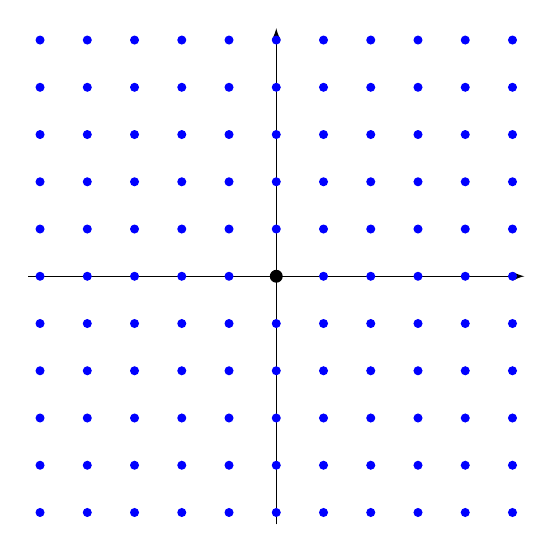
\begin{tikzpicture}[scale=0.3]
		\coordinate (Origin)   at (0,0);
		\coordinate (XAxisMin) at (-10.5,0);
		\coordinate (XAxisMax) at (10.5,0);
		\coordinate (YAxisMin) at (0,-10.5);
		\coordinate (YAxisMax) at (0,10.5);
		\draw [thin, black,-latex] (XAxisMin) -- (XAxisMax);% Draw x axis
		\draw [black,-latex] (YAxisMin) -- (YAxisMax);% Draw y axis

		\clip (-10.5,-10.5) rectangle (10.5cm,10.5cm); % Clips the picture...
		
		\foreach \x in {-5,-4,...,5}{% Two indices running over each
		  \foreach \y in {-5,-4,...,5}{% node on the grid we have drawn 
			\node[draw,circle,inner sep=1pt,fill, blue] at (2*\x,2*\y) {};
				% Places a dot at those points
		  }
		}
		\node[draw,circle,inner sep=1.5pt,fill, black] at (0,0) {};
	  \end{tikzpicture}
	  \caption{The ring of integers $\mathbb{Z}[i]$ for $\mathbb{Q}(i)$.}
	  \label{fig:gaussian-1}
	\end{figure}
	
	\begin{figure}[ht]
	\centering
	  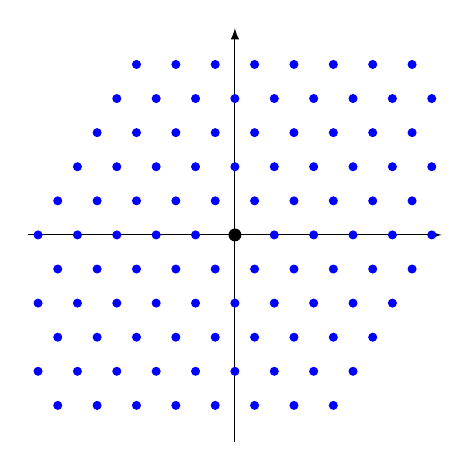
\begin{tikzpicture}[scale=0.25]
		\coordinate (Origin)   at (0,0);
		\coordinate (XAxisMin) at (-10.5,0);
		\coordinate (XAxisMax) at (10.5,0);
		\coordinate (YAxisMin) at (0,-10.5);
		\coordinate (YAxisMax) at (0,10.5);
		\draw [thin, black,-latex] (XAxisMin) -- (XAxisMax);% Draw x axis
		\draw [black,-latex] (YAxisMin) -- (YAxisMax);% Draw y axis

		\clip (-10.5,-10.5) rectangle (10.5cm,10.5cm); % Clips the picture...
	
		\foreach \x in {-5,-4,...,5}{% Two indices running over each
		  \foreach \y in {-5,-4,...,5}{% node on the grid we have drawn 
			\node[draw,circle,inner sep=1pt,fill, blue] at (2*\x+\y,1.732*\y) {};
				% Places a dot at those points
		  }
		}
		\node[draw,circle,inner sep=1.5pt,fill, black] at (0,0) {};
	  \end{tikzpicture}
	  \caption{The ring of integers $\mathbb{Z}[\frac{1+\sqrt{-3}}{2}]$ for $\mathbb{Q}(\sqrt{-3})$.}
	  \label{fig:eisenstein-1}
	\end{figure}
	
	In particular, we observe that each of these rings of integers is a lattice in $\mathbb{R}^2$.  On the other hand, $\mathbb{Q}(\sqrt{5})$ most naturally embeds into $\mathbb{R}$, not $\mathbb{R}^2$.  It turns out (not entirely obviously) that the ring of integers $\mathbb{Z}[\frac{1+\sqrt{5}}{2}]$ is dense in $\mathbb{R}$; see Figure \ref{fig:sqrt-5-1}.
	
	\begin{figure}[h]
	\centering
	  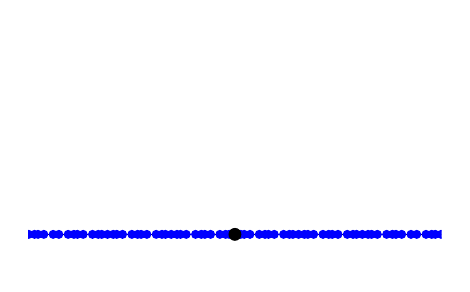
\begin{tikzpicture}[scale=0.25]
		\coordinate (Origin)   at (0,0);
		\coordinate (XAxisMin) at (-10.5,0);
		\coordinate (XAxisMax) at (10.5,0);
		\coordinate (YAxisMin) at (0,-10.5);
		\coordinate (YAxisMax) at (0,10.5);
		\draw [thin, black,-latex] (XAxisMin) -- (XAxisMax);% Draw x axis
		%\draw [black,-latex] (YAxisMin) -- (YAxisMax);% Draw y axis

		\clip (-10.5,-1.5) rectangle (10.5cm,10.5cm); % Clips the picture...

		\foreach \x in {-5,-4,...,5}{% Two indices running over each
		  \foreach \y in {-5,-4,...,5}{% node on the grid we have drawn 
			\node[draw,circle,inner sep=1pt,fill, blue] at (2*\x+\y+\y*2.236,0) {};
				% Places a dot at those points
		  }
		}
		\node[draw,circle,inner sep=1.5pt,fill, black] at (0,0) {};
	  \end{tikzpicture}
	  \caption{A (bad!) visualization of the ring of integers $\mathbb{Z}[\frac{1+\sqrt{5}}{2}]$ of $\mathbb{Q}(\sqrt{5})$ on the number line.}
	  \label{fig:sqrt-5-1}
	\end{figure}
	
	Our first goal is to provide a way of visualizing $\mathbb{Z}[\frac{1+\sqrt{5}}{2}]$ as a lattice, analogous to Figures \ref{fig:gaussian-1} and \ref{fig:eisenstein-1}.  For this, we need the notion of \emph{embeddings}.
	
	\begin{definition}
		A real embedding of a number field $K$ is an injective homomorphism $\sigma\colon K \hookrightarrow \mathbb{R}$.  A complex embedding of a number field $K$ is an injective homomorphism $\sigma\colon K \hookrightarrow \mathbb{C}$ that doesn't factor through an embedding to $\mathbb{R}$ (equivalently, whose image $\sigma(K)$ is not contained in $\mathbb{R}$).  An embedding of $K$ is implicitly either a real or complex embedding.
	\end{definition}
	
	We summarize several useful facts in the following lemma.
	
	\begin{lemma}\label{lem:embedding-props}
		Let $K$ be a number field of degree $n$.  Then:
		\begin{enumerate}
			\item If $\alpha \in K$ is a root of $f \in \mathbb{Q}[x]$, then so is $\sigma(\alpha)$.
			\item There are exactly $n$ embeddings of $K$.
			\item Complex embeddings come in pairs, differing by complex conjugation.  
			\item If $r_1$ denotes the number of real embeddings of $K$ and $r_2$ denotes the number of pairs of complex embeddings, then $n=r_1+2r_2$.
			\item If $\widetilde{K}$ denotes the normal closure\footnote{i.e., splitting field} of $K$, then $\mathrm{Gal}(\widetilde{K}/\mathbb{Q})$ acts faithfully and transitively on the set of embeddings of $K$.
		\end{enumerate}
	\end{lemma}
	\begin{proof}
		1) Since $\sigma$ is an injective field homomorphism, it fixes $\mathbb{Q}$.  Thus, for any $f \in \mathbb{Q}[x]$ and any $\alpha \in K$, $\sigma(f(\alpha)) = f(\sigma(\alpha))$, so $\sigma(\alpha)$ is a root of $f$ if and only if $\alpha$ is.
		
		2) Since $K$ has degree $n$, there is some $\alpha$ for which $K = \mathbb{Q}(\alpha)$ and whose minimal polynomial $f_\alpha(x)$ has degree $n$.  By part 1), $\sigma(\alpha)$ must be one of the $n$ conjugates of $\alpha$, and this choice completely determines $\sigma$ since $\sigma$ must fix $\mathbb{Q}$.  Each of these $n$ choices defines an embedding, and thus there are exactly $n$ embeddings of $K$.
		
		3) Let $\tau$ denote complex conjugation.  If $\sigma$ is a complex embedding, then $\tau \circ \sigma$ is also an embedding of $K$, necessarily not equal to $\sigma$ since $\sigma$ is complex.
		
		4) Follows from 2) and 3).
		
		5)  By 1) and 2), if $K = \mathbb{Q}(\alpha)$, then embeddings of $K$ are in correspondence with a choice $\sigma(\alpha) = \alpha_i$, where $\alpha_1,\dots,\alpha_n$ are the conjugates of $\alpha$.  Moreover, $\widetilde{K}=\mathbb{Q}(\alpha_1,\dots,\alpha_n)$, so all $\alpha_i$ are defined in $\widetilde{K}$.  An element $\phi \in \mathrm{Gal}(\widetilde{K}/\mathbb{Q})$ is a field automorphism of $\widetilde{K}$, which must send each $\alpha_i$ to some $\alpha_j$.  That is, it acts on the set $\{\alpha_1,\dots,\alpha_n\}$.  It therefore also acts in the obvious way on the set of embeddings by exploiting the correspondence between embeddings and conjugates.  
		
		A ``transitive'' action of a group $G$ on a set $\{1,\dots,n\}$ is one for which, for every pair $(i,j)$, there is an element $g \in G$ for which $g(i)=j$.  There is a field automorphism $\phi \in \mathrm{Gal}(\widetilde{K}/\mathbb{Q})$ for which $\phi(\alpha) = \alpha_i$ for any $i$, from which follows that the action of $\mathrm{Gal}(\widetilde{K}/\mathbb{Q})$ on the set of conjugates of $\alpha$ is transitive.  By the way we defined the action on the set of embeddings, it follows that the action of $\mathrm{Gal}(\widetilde{K}/\mathbb{Q})$ on the set of embeddings is also transitive.
		
		An action is ``faithful'' if only the identity element fixes everything.  The action of $\mathrm{Gal}(\widetilde{K}/\mathbb{Q})$ on the conjugates $\alpha_1,\dots,\alpha_n$ is faithful: if $\phi(\alpha_i) = \alpha_i$ for each $i$, then since $\widetilde{K}=\mathbb{Q}(\alpha_1,\dots,\alpha_n)$, $\phi$ must be the identity automorphism.  Since we have defined the action of $\mathrm{Gal}(\widetilde{K}/\mathbb{Q})$ on embeddings via its action on conjugates, it follows that the action of $\mathrm{Gal}(\widetilde{K}/\mathbb{Q})$ on the set of embeddings must be faithful as well.
	\end{proof}
	
	\begin{remark}
		There's a lot of formal manipulation going on in the statement and proof of the fifth claim.  There are two main points.  First, we can abstractly construct number fields as quotients $\mathbb{Q}[x] / (f(x))$ where $f(x)$ is an irreducible polynomial, but in this formalism we haven't ``picked a root.''  For example, if $f(x)=x^2-2$, then we have formally constructed $\mathbb{Q}(\sqrt{2}) \simeq \mathbb{Q}[x]/(x^2-2)$ without having to specify which squareroot of $2$ we mean.  We can let embeddings ``choose'' a squareroot for us.  The substance of the fifth point is entirely that instead of the (very useful!) notion that the Galois group permutes roots of irreducible polynomials, it instead permutes the embeddings.  In modern number theory, it's considered gauche to fix a root when thinking about number fields.  You'll never actually be misled if you want to fix a root, but it's both psychologically and mathematically important to remember you could have made a different choice, and that embeddings create the universes in which you made that alternate choice.  
		
		The other thing it's important to extract from this is that it gives a ``element free'' way of thinking about the Galois group.  For us, this will be important in situations where we have something like $K = \mathbb{Q}(\alpha) = \mathbb{Q}(\beta)$, where we care about both $\alpha$ and $\beta$.  Viewing the Galois group as acting on the embeddings of $K$ gives a consistent way to view it acting on the conjugates of $\alpha$ and $\beta$ simultaneously.  If we label the $n$ embeddings of $K$ as $\sigma_1,\dots\sigma_n$ and define $\alpha_i = \sigma_i(\alpha)$ and $\beta_i = \sigma_i(\beta)$, then the permutation actions of the Galois group on $\{\alpha_1,\dots,\alpha_n\}$ and $\{\beta_1,\dots,\beta_n\}$ must be identical.
	\end{remark}
	
	The claim that the complex embeddings can be paired according to whether they differ by complex conjugation is important.  Loosely, you should think of these embeddings as giving you the same information about $K$ as each other.  By contrast, two real embeddings never give the same information as each other.  (They're more different than two conjugate complex embeddings in some intrinsic sense.)  We therefore introduce a definition that tracks the number of ``interesting'' embeddings of a field.
	
	\begin{definition}
		If $K$ is a number field, then its \emph{signature} is the pair $(r_1,r_2)$, where $r_1$ is the number of real embeddings of $K$ and $r_2$ is the number of pairs of complex embeddings of $K$.
	\end{definition}
	
	For example, both $\mathbb{Q}(i)$ and $\mathbb{Q}(\sqrt{-3})$ have signature $(0,1)$, which indicates they have only $0+1=1$ ``interesting'' embedding (which is complex).  We've implicitly used this embedding in generating Figures \ref{fig:gaussian-1} and \ref{fig:eisenstein-1}.  By contrast, $\mathbb{Q}(\sqrt{5})$ has signature $(2,0)$, so it has two interesting embeddings -- and we only used one of these in generating Figure \ref{fig:sqrt-5-1}.  Thus, we've left out some interesting information about $\mathbb{Q}(\sqrt{5})$, and that's why the picture turns out to be bad.  To correct this, we'll need to use both embeddings of $\mathbb{Q}(\sqrt{5})$.  We introduce a general definition first, then see how it resolves this situation for $\mathbb{Q}(\sqrt{5})$.
	
	\begin{definition}
		If $K$ is a number field with signature $(r_1,r_2)$, then its \emph{Minkowski embedding} $\iota\colon K \hookrightarrow \mathbb{R}^n$ is defined as follows.  Let $\sigma_1,\dots,\sigma_{r_1}$ denote the real embeddings of $K$, and let $\sigma_{r_1+1},\dots,\sigma_{r_1+r_2}$ denote a representative from each pair of complex embeddings.  The embedding $\iota\colon K \hookrightarrow \mathbb{R}^{r_1} \oplus \mathbb{C}^{r_2} \simeq \mathbb{R}^n$ is then defined by
			\[
				\iota(x) := (\sigma_1(x),\dots,\sigma_{r_1}(x),\sigma_{r_1+1}(x),\dots,\sigma_{r_1+r_2}(x)).
			\]
	\end{definition}
	
	For $K=\mathbb{Q}(\sqrt{5})$, the two real embeddings correspond to choosing between $\sqrt{5}$ and $-\sqrt{5}$, and the Minkowski embedding is given by $\iota(a+b\sqrt{5}) = (a + b\sqrt{5}, a-b\sqrt{5}) \in \mathbb{R}^2$.  With this embedding, we find the ring of integers $\mathbb{Z}[\frac{1+\sqrt{5}}{2}]$ is again a lattice in $\mathbb{R}^2$; see Figure \ref{fig:sqrt-5-2}.
	
	\begin{figure}[ht]
	\centering
	  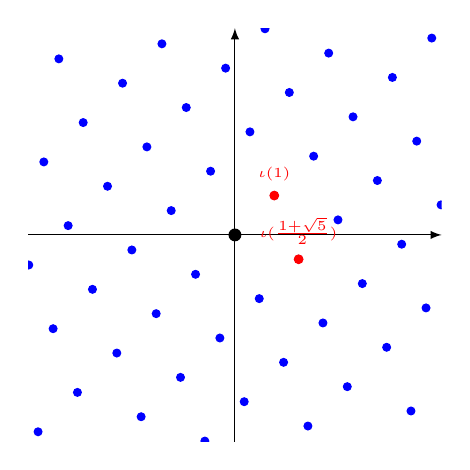
\begin{tikzpicture}[scale=0.25]
		\coordinate (Origin)   at (0,0);
		\coordinate (XAxisMin) at (-10.5,0);
		\coordinate (XAxisMax) at (10.5,0);
		\coordinate (YAxisMin) at (0,-10.5);
		\coordinate (YAxisMax) at (0,10.5);
		\draw [thin, black,-latex] (XAxisMin) -- (XAxisMax);% Draw x axis
		\draw [black,-latex] (YAxisMin) -- (YAxisMax);% Draw y axis

		\clip (-10.5,-10.5) rectangle (10.5cm,10.5cm); % Clips the picture...
	
		\foreach \x in {-5,-4,...,5}{% Two indices running over each
		  \foreach \y in {-5,-4,...,5}{% node on the grid we have drawn 
			\node[draw,circle,inner sep=1pt,fill, blue] at (2*\x+\y*3.236,2*\x-1.236*\y) {};
				% Places a dot at those points
		  }
		}
		\node[label={\tiny \color{red} $\iota(1)$},draw,circle,inner sep=1.1pt,fill, red] at (2,2) {};
		\node[label={\tiny \color{red} $\iota(\frac{1+\sqrt{5}}{2})$},draw,circle,inner sep=1.1pt,fill, red] at (3.236,-1.236) {};
		\node[draw,circle,inner sep=1.5pt,fill, black] at (0,0) {};
	  \end{tikzpicture}
	  \caption{The Minkowski embedding of the ring of integers $\mathbb{Z}[\frac{1+\sqrt{5}}{2}]$ for $\mathbb{Q}(\sqrt{5})$.}
	  \label{fig:sqrt-5-2}
	\end{figure}
	
	Analogous pictures hold for the ring of integers in any quadratic field using the Minkowski embedding.  In fact, this holds much more generally.
	
	\begin{proposition}
		If $K$ is a number field of degree $n$, then its ring of integers $\mathcal{O}_K$ is a lattice in $\mathbb{R}^n$ under the Minkowksi embedding.
	\end{proposition}
	
	We'll discuss this in degrees greater than $2$ soon, but first, we consider an important notion that's naturally attached to a ring of integers, namely, its discriminant.
	
\subsection{Discriminants}
		
	We've now attached to a number field $K$ its ring of integers, and we've found that we can visualize the ring of integers as a lattice in $\mathbb{R}^n$.  We now want some notion that measures how complicated this ring of integers is.  The most basic invariant attached to a lattice $\Lambda \subseteq \mathbb{R}^n$ is its covolume, which measures the volume (or area) of a fundamental parallelotope for the lattice.  A \emph{fundemantal parallelotope} is a nice choice of a region representing the quotient $\mathbb{R}^n/\Lambda$.  We consider this notion first in the case $n=2$.
	
	As we've seen, when $n=2$, the ring of integers in a quadratic field $K$ is given by $\mathcal{O}_K = \mathbb{Z}[\alpha] = \mathbb{Z} \oplus \mathbb{Z}\alpha$.  A fundamental parallelotope (or, in this case, a fundamental parallelogram) for 
	a lattice $\Lambda = \mathbb{Z}v_1 \oplus \mathbb{Z}v_2 \subseteq \mathbb{R}^2$ with $v_1,v_2 \in \mathbb{R}^2$ is the set $\{c_1v_1 + c_2v_2 : 0 \leq c_1,c_2 < 1\}$.  For the rings of integers we've considered, this is shown in Figures \ref{fig:gaussian-2}--\ref{fig:sqrt-5-3} below.
	
	\begin{figure}[ht]
	\centering
	  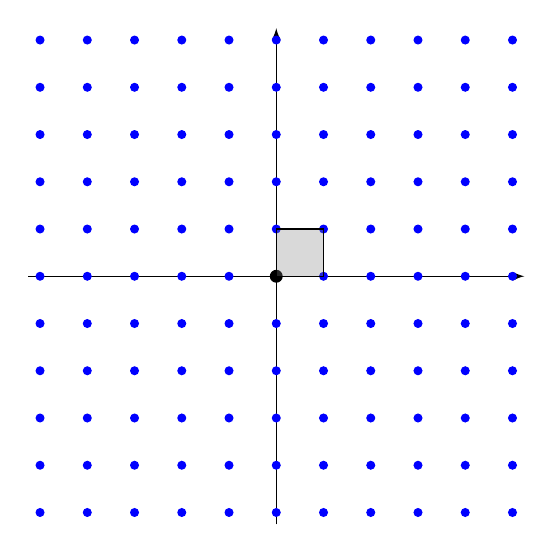
\begin{tikzpicture}[scale=0.3]
		\coordinate (Origin)   at (0,0);
		\coordinate (XAxisMin) at (-10.5,0);
		\coordinate (XAxisMax) at (10.5,0);
		\coordinate (YAxisMin) at (0,-10.5);
		\coordinate (YAxisMax) at (0,10.5);
		\draw [thin, black,-latex] (XAxisMin) -- (XAxisMax);% Draw x axis
		\draw [black,-latex] (YAxisMin) -- (YAxisMax);% Draw y axis

		\clip (-10.5,-10.5) rectangle (10.5cm,10.5cm); % Clips the picture...

		\foreach \x in {-5,-4,...,5}{% Two indices running over each
		  \foreach \y in {-5,-4,...,5}{% node on the grid we have drawn 
			\node[draw,circle,inner sep=1pt,fill, blue] at (2*\x,2*\y) {};
				% Places a dot at those points
		  }
		}
		\node[draw,circle,inner sep=1.5pt,fill, black] at (0,0) {};
		\filldraw[fill=gray, fill opacity=0.3, draw=black] (Origin)
			rectangle (2,2);
	  \end{tikzpicture}
	  \caption{The fundamental parallelotope for $\mathbb{Z}[i]$.}
	  \label{fig:gaussian-2}
	\end{figure}
	
	\begin{figure}[ht]
	\centering
	  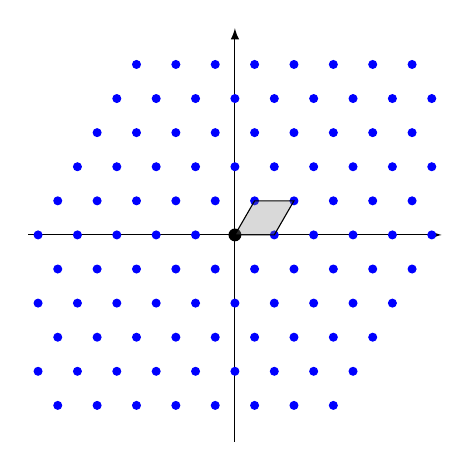
\begin{tikzpicture}[scale=0.25]
		\coordinate (Origin)   at (0,0);
		\coordinate (XAxisMin) at (-10.5,0);
		\coordinate (XAxisMax) at (10.5,0);
		\coordinate (YAxisMin) at (0,-10.5);
		\coordinate (YAxisMax) at (0,10.5);
		\draw [thin, black,-latex] (XAxisMin) -- (XAxisMax);% Draw x axis
		\draw [black,-latex] (YAxisMin) -- (YAxisMax);% Draw y axis

		\clip (-10.5,-10.5) rectangle (10.5cm,10.5cm); % Clips the picture...

		\foreach \x in {-5,-4,...,5}{% Two indices running over each
		  \foreach \y in {-5,-4,...,5}{% node on the grid we have drawn 
			\node[draw,circle,inner sep=1pt,fill, blue] at (2*\x+\y,1.732*\y) {};
				% Places a dot at those points
		  }
		}
		\node[draw,circle,inner sep=1.5pt,fill, black] at (0,0) {};
		\filldraw[fill=gray, fill opacity=0.3, draw=black] (0,0) -- (1,1.732) -- (3,1.732) -- (2,0) -- cycle;
	  \end{tikzpicture}
	  \caption{The fundamental parallelotope for $\mathbb{Z}[\frac{1+\sqrt{-3}}{2}]$.}
	  \label{fig:eisenstein-2}
	\end{figure}
	
	\begin{figure}[ht]
	\centering
	  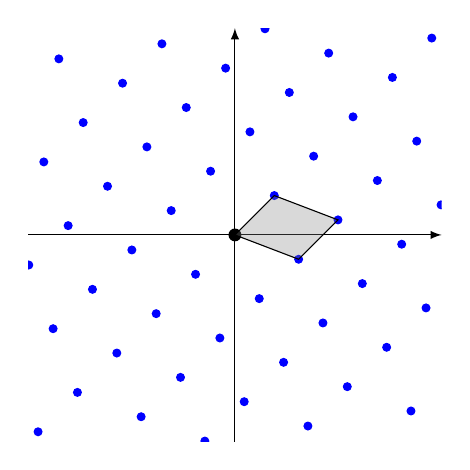
\begin{tikzpicture}[scale=0.25]
		\coordinate (Origin)   at (0,0);
		\coordinate (XAxisMin) at (-10.5,0);
		\coordinate (XAxisMax) at (10.5,0);
		\coordinate (YAxisMin) at (0,-10.5);
		\coordinate (YAxisMax) at (0,10.5);
		\draw [thin, black,-latex] (XAxisMin) -- (XAxisMax);% Draw x axis
		\draw [black,-latex] (YAxisMin) -- (YAxisMax);% Draw y axis

		\clip (-10.5,-10.5) rectangle (10.5cm,10.5cm); % Clips the picture...
	
		\foreach \x in {-5,-4,...,5}{% Two indices running over each
		  \foreach \y in {-5,-4,...,5}{% node on the grid we have drawn 
			\node[draw,circle,inner sep=1pt,fill, blue] at (2*\x+\y*3.236,2*\x-1.236*\y) {};
				% Places a dot at those points
		  }
		}
		\node[draw,circle,inner sep=1.5pt,fill, black] at (0,0) {};
		\filldraw[fill=gray, fill opacity=0.3, draw=black] (0,0) -- (2,2) -- (5.235,0.764) -- (3.236,-1.236) -- cycle;
	  \end{tikzpicture}
	  \caption{The fundamental parallelotope for $\mathbb{Z}[\frac{1+\sqrt{5}}{2}]$.}
	  \label{fig:sqrt-5-3}
	\end{figure}
	
	We now want to understand the volume of this fundamental parallelotope (which, in this case, is just its area).  By definition, this is the \emph{covolume} of $\mathcal{O}_K$, which we denote $\mathrm{covol}(\mathcal{O}_K) = \mathrm{vol}(\mathbb{R}^2/\mathcal{O}_K)$.  We could do this by hand if we're sufficiently careful, but in general, if $v_1,\dots,v_n$ are (row) vectors in $\mathbb{R}^n$, the volume of the parallelotope formed by is the absolute value of the determinant of the $n\times n$ matrix formed by $v_1,\dots,v_n$.
	
	For the ring of integers $\mathcal{O}_K = \mathbb{Z}[\frac{1+\sqrt{5}}{2}]$ of $K = \mathbb{Q}(\sqrt{5})$ -- the hardest of the examples to do by hand -- the associated $v_1$ and $v_2$ are simply $\iota(1)=(1,1)$ and $\iota\left(\frac{1+\sqrt{5}}{2}\right) = (\frac{1+\sqrt{5}}{2}, \frac{1-\sqrt{5}}{2})$.  Thus, we find
		\[
			\mathrm{covol}( \mathcal{O}_K)
				= \left| \det \begin{pmatrix}
					1 & 1 \\
					\frac{1+\sqrt{5}}{2} & \frac{1-\sqrt{5}}{2} \end{pmatrix} \right|
				= \sqrt{5}.
		\]
	This is entirely representative of the situation for real quadratic fields: if $\mathcal{O}_K = \mathbb{Z}[\alpha]$, then
		\[
			\mathrm{covol}(\mathcal{O}_K)
				= \left| \det \begin{pmatrix} 1 & 1 \\ \sigma_1(\alpha) & \sigma_2(\alpha) \end{pmatrix} \right|.
		\]
	The absolute value in this formula is necessary for a couple of reasons.  First, the determinant outputs a ``signed'' area or signed volume, that pays attention to the orientation of the basis vectors.  Second, in principle we could have chosen the two real embeddings in the opposite order -- remember, there's no algebraically preferred squareroot -- and we'd want our answer to be the same regardless.  Swapping those two embeddings would also institute a sign ambiguity, since it would have the effect of swapping the two columns.  Thus, the absolute value resolves these two different sign ambiguities.  However, there is something else we could have done to resolve the sign (namely, squaring the determinant), and it's this other resolution that's of more intrinsic interest.
	
	\begin{definition}
		The \emph{discriminant} of a quadratic field $K$ with ring of integers $\mathcal{O}_K = \mathbb{Z}[\alpha]$ is defined to be
			\[
				\mathrm{Disc}(K)
					= \det\begin{pmatrix} 1 & 1 \\ \sigma_1(\alpha) & \sigma_2(\alpha) \end{pmatrix}^2,
			\]
		where $\sigma_1$ and $\sigma_2$ are the two embeddings of $K$.
	\end{definition}
	
	Notice that we've given this definition for both real and complex quadratic fields, even though we motivated it only for real quadratic fields.  We'll discuss how it relates to the covolume of $\mathcal{O}_K$ for complex quadratic fields shortly, but first, we have an important lemma.
	
	\begin{lemma}\label{lem:disc-in-Z-quadratic}
		For any quadratic field, $\mathrm{Disc}(K)$ is an integer (i.e., $\mathrm{Disc}(K) \in \mathbb{Z}$).
	\end{lemma}
	\begin{proof}
		Given the formula for $\alpha$ in Lemma \ref{lem:quadratic-integers}, we could approach this directly.  Instead, we give a slightly more roundabout proof that will be useful when we define discriminants for higher degree fields.
		In particular, we will first show that $\mathrm{Disc}(K)$ is an \emph{algebraic} integer.  We will then show that it is also rational, so it must be in the ring of integers of $\mathbb{Q}$, which is just $\mathbb{Z}$.
		
		To see that $\mathrm{Disc}(K)$ is an algebraic integer, notice that every entry in the matrix defining the discriminant is an algebraic integer.  The determinant is built by certain sums of products of these entries, and thus must be an algebraic integer as well by Lemma \ref{lem:integers-closed}.  Again by Lemma \ref{lem:integers-closed}, we conclude that $\mathrm{Disc}(K)$ is an algebraic integer as claimed.
		
		To see that $\mathrm{Disc}(K) \in \mathbb{Q}$, we use Galois theory.  By Lemma \ref{lem:embedding-props}(5), the Galois group $\mathrm{Gal}(K/\mathbb{Q})$ acts on the embeddings of $K$.  If we apply an element $\phi \in \mathrm{Gal}(K/\mathbb{Q})$ to $\mathrm{Disc}(K)$, it follows that the resulting matrix will have its columns permuted according to how $\phi$ acts on the embeddings.  If $\phi$ is the nontrivial element of $\mathrm{Gal}(K/\mathbb{Q})$, the resulting matrix will have its determinant changed by $-1$.  Consequently, we find $\phi(\mathrm{Disc}(K)) = (-1)^2 \mathrm{Disc}(K) = \mathrm{Disc}(K)$.  In particular, $\mathrm{Disc}(K)$ is fixed by every element of $\mathrm{Gal}(K/\mathbb{Q})$.  By the Galois correspondence, the only elements of $K$ fixed by every element of the Galois group are those in $\mathbb{Q}$.  We therefore conclude that $\mathrm{Disc}(K) \in \mathbb{Q}$, and thus also that $\mathrm{Disc}(K) \in \mathbb{Z}$ as indicated above.
	\end{proof}
	
	We now connect this definition back to covolumes for both real and complex quadratic fields.
	
	\begin{lemma}\label{lem:covolume-quadratic}
		Let $K$ be a quadratic field with ring of integers $\mathcal{O}_K$ and signature $(r_1,r_2)$.  Then
			\[
				\mathrm{covol}(\mathcal{O}_K)
					= 2^{-r_2} \sqrt{|\mathrm{Disc}(K)|}.
			\]
		In particular, if $K$ is real, then $\mathrm{covol}(\mathcal{O}_K) = \sqrt{|\mathrm{Disc}(K)|}$, and if $K$ is complex, then $\mathrm{covol}(\mathcal{O}_K) = \frac{1}{2} \sqrt{|\mathrm{Disc}(K)|}$.
	\end{lemma}
	\begin{proof}
		If $K$ is real, then this follows from the definition of the discriminant, as indicated in the discussion prior to that definition.\footnote{Notice also that discussion implies the discriminant of a real quadratic field is positive, since it's the square of a real number (namely, a signed area).  That means $\mathrm{covol}(\mathcal{O}_K) = \sqrt{\mathrm{Disc}(K)}$ in this case, which is what you might have expected to see here.}  Thus, we focus on the case of complex quadratic fields.  We give a bare hands proof, but there are more abstract, high-brow ways of seeing this.
		
		In this case, if $\mathcal{O}_K = \mathbb{Z}[\alpha]$, we may write $\alpha = a + bi$, with $a$ and $b$ real.  Then, in the Minkowski embedding, $\iota(\mathcal{O}_K)$ has basis vectors $v_1$ and $v_2$ given by $v_1 = (1,0)$ and $v_2 = (a,b)$.  (Compare this with Figures \ref{fig:gaussian-1} and \ref{fig:eisenstein-1}, for example.)  Thus, the covolume is given by
			\[
				\mathrm{covol}(\mathcal{O}_K)
					= \left| \det \begin{pmatrix} 1 & 0 \\ a & b \end{pmatrix} \right| = |b|.
			\]
		On the other hand, the matrix defining the discriminant has
			\[
				\det \begin{pmatrix} 1 & 1 \\ a+bi & a-bi \end{pmatrix} = 2bi.
			\]
		Thus, $\mathrm{Disc}(K) = -4b^2$, from which follows the claim.
	\end{proof}
	
	Before turning to higher degree fields, we note that it is possible to explicitly determine the discriminant of quadratic fields.
	
	\begin{lemma}\label{lem:quadratic-discriminant}
		Suppose $K = \mathbb{Q}(\sqrt{d})$ for some squarefree $d \ne 1$.  Then
			\[
				\mathrm{Disc}(K) =
					\begin{cases}
						d, & \text{if } d \equiv 1 \pmod{4}, \\
						4d, & \text{if } d \equiv 2,3 \pmod{4}.
					\end{cases}
			\]
		In particular, $\mathrm{Disc}(K)>0$ if $K$ is real quadratic, and $\mathrm{Disc}(K)<0$ if $K$ is complex quadratic.
	\end{lemma}
	
\subsection{Higher degree extensions}

	The story for higher degree extensions is very similar: the ring of integers forms a lattice in $\mathbb{R}^n$ with covolume $2^{-r_2} \sqrt{|\mathrm{Disc}(K)|}$ (with an analogous definition of the discriminant).  Unfortunately, though, there is one substantial complication.  In particular, it is no longer generally the case that the ring of integers $\mathcal{O}_K$ in fields of degree $n > 2$ is of the form $\mathbb{Z}[\alpha]$.  Instead, we often need multiple generators, a priori up to $n-1$.  Intuitively, you should be thinking of something like the following.  If $K = \mathbb{Q}(\alpha)$, then the Minkowski embeddings $\iota(1),\iota(\alpha),\dots,\iota(\alpha^{n-1})$ will be linearly independent in $\mathbb{R}^n$, so generate \emph{some} lattice in $\mathbb{R}^n$, but there's no particular reason to expect it should be possible to make that lattice the full ring of integers.  If $n=2$, then we're only looking at the vectors $\iota(1),\iota(\alpha)$, and it's hopefully believable that there should be a ``best possible'' $\alpha \in \mathcal{O}_K$ to use to generate the full ring of integers.  (This is what Lemma \ref{lem:quadratic-integers} is doing.)  For higher degrees, say $n=3$, we'd need to argue something like, it's possible to choose a ``best possible'' $\alpha$ such that $\alpha^2$ is also ``best possible.''  That should sound hard to do!  For some fields, it is possible, while for others, it's not.
	
	\begin{example}
		1) Let $\alpha$ be a root of $x^3+4x^2+3x+8$.  Then $K=\mathbb{Q}(\alpha)$ is a cubic field, but $\mathcal{O}_K = \mathbb{Z}[\alpha, \frac{\alpha^2+\alpha}{2}]$, and $\mathcal{O}_K \ne \mathbb{Z}[\beta]$ for any $\beta \in \mathcal{O}_K$.
		
		2) Let $\alpha$ be a root of $x^3+x+1$.  Then $K = \mathbb{Q}(\alpha)$ is a cubic field, and $\mathcal{O}_K = \mathbb{Z}[\alpha]$.  So this can happen!
	\end{example}

	\begin{remark}
		If the ring of intgers $\mathcal{O}_K$ of a field $K$ is of the form $\mathcal{O}_K = \mathbb{Z}[\alpha]$ (like it is in the second example) then we sometimes say $K$ is \emph{monogenic}.  It is an open problem to determine even how many cubic fields are monogenic, but it is generally expected that asymptotically $0\%$ of cubic fields will be monogenic (or in any degree $n \geq 3$).  The fact that this is an open problem should hopefully indicate that this is a subtle issue.
	\end{remark}
	
	This brings us to an important definition for higher degree fields.
	
	\begin{definition}
		If $K$ is a degree $n$ field, then an \emph{integral basis} for $\mathcal{O}_K$ is any set $\{\alpha_1,\dots,\alpha_n\} \subseteq \mathcal{O}_K$ for which
			\[
				\mathcal{O}_K = \mathbb{Z}\alpha_1 \oplus \dots \oplus \mathbb{Z}\alpha_n.
			\]
		Equivalently, an integral basis is a basis for $\mathcal{O}_K$ as a lattice under the Minkowski embedding.
	\end{definition}
	
	\begin{example}
		Returning to our two example cubic fields, we find that $\{1,\alpha, \frac{\alpha^2+\alpha}{2}\}$ is an integral basis for the first, while $\{1,\alpha,\alpha^2\}$ is an integral basis for the second.
	\end{example}
	
	We next note that, even in the case that $K$ is not monogenic, the ring of integers can't be \emph{too} far from rings $\mathbb{Z}[\alpha]$.
	
	\begin{lemma}
		If $K = \mathbb{Q}(\alpha)$ for some algebraic integer $\alpha$, then $\mathcal{O}_K \supseteq \mathbb{Z}[\alpha]$, and the index $[\mathcal{O}_K : \mathbb{Z}[\alpha]]$ is finite.
	\end{lemma}
	\begin{proof}
		For the first claim, since $\alpha$ is an algebraic integer in $K$, $\alpha \in \mathcal{O}_K$, and thus $\mathbb{Z}[\alpha] \subseteq \mathcal{O}_K$ since $\mathcal{O}_K$ is a ring.
		
		For the second, since $K = \mathbb{Q}(\alpha)$, the set $\{1,\alpha,\dots,\alpha^{n-1}\}$ is a $\mathbb{Q}$-basis for $K$.  Consequently, every element in an integral basis for $\mathcal{O}_K$ can be expressed rationally in terms of $\{1,\alpha,\dots,\alpha^{n-1}\}$.  Taking the least common multiple of the denominators in these expressions, we see that there is some integer $m \geq 1$ such that $\mathcal{O}_K \subseteq \frac{1}{m} \mathbb{Z}[\alpha]$.  Equivalently, we find $m \mathcal{O}_K \subseteq \mathbb{Z}[\alpha]$.  The index $[\mathcal{O}_K : m\mathcal{O}_K] = m^n$ is finite, so the index $[\mathcal{O}_K : \mathbb{Z}[\alpha]]$ must be finite too.
	\end{proof}
	
	We now record a few useful facts about integral bases.
	
	\begin{proposition} \label{prop:integral-basis}
		Let $K$ be a number field.
		
		1) There is always an integral basis of $\mathcal{O}_K$ containing $1$.
		
		2)  Any two integral bases $\{\alpha_1,\dots,\alpha_n\}$ and $\{\beta_1,\dots,\beta_n\}$ differ by an invertible linear change of variables over $\mathbb{Z}$.  Equivalently, there is some matrix $M \in \mathrm{GL}_n(\mathbb{Z})$ such that 
			\[
				\begin{pmatrix} \alpha_1 \\ \vdots \\ \alpha_n \end{pmatrix} = M \begin{pmatrix} \beta_1 \\ \vdots \\ \beta_n\end{pmatrix}.
			\]
	\end{proposition}
	\begin{proof}
		The second claim follows from parsing the definition of integral bases and the matrix multiplication formula.  The first isn't entirely obvious, and the proof isn't especially illuminating (at least to me!) but it's useful to know.
	\end{proof}
	
	Recall that an $n\times n$ matrix is in $\mathrm{GL}_n(\mathbb{Z})$ precisely when its determinant is $\pm 1$.  Finally, then, we come to the general definition of a discriminant.
	
	\begin{definition}
		Let $K$ be a degree $n$ number field, and let $\{\alpha_1,\dots,\alpha_n\}$ be any integral basis for $\mathcal{O}_K$.  We define the \emph{discriminant} of $K$ by
			\[
				\mathrm{Disc}(K) = \det\begin{pmatrix}
					\sigma_1(\alpha_1) & \dots & \sigma_n(\alpha_1) \\
					\vdots & & \vdots \\
					\sigma_1(\alpha_n) & \dots & \sigma_n(\alpha_n)
				\end{pmatrix}^2.
			\]
		Here, the rows are indexed by the different elements of the integral basis, and the columns are indexed by the $n$ embeddings $\sigma_1,\dots,\sigma_n$ of $K$.
	\end{definition}

	\begin{lemma}
		Let $K$ be a number field.
		
		1) The definition of $\mathrm{Disc}(K)$ given above does not depend on the choice of integral basis $\{\alpha_1,\dots,\alpha_n\}$.
		
		2) For any $K$, $\mathrm{Disc}(K) \in \mathbb{Z}$.
	\end{lemma}
	\begin{proof}
		1) Let $\{\alpha_1,\dots,\alpha_n\}$ and $\{\beta_1,\dots,\beta_n\}$ be two integral bases, and let $\mathrm{Disc}_\alpha(K)$ and $\mathrm{Disc}_\beta(K)$ be the discriminants defined with respect to the two bases.  Thus, we wish to show $\mathrm{Disc}_\alpha(K) = \mathrm{Disc}_\beta(K)$.  Let $M \in \mathrm{GL}_n(\mathbb{Z})$ be the matrix guaranteed by Proposition \ref{prop:integral-basis}. Then
			\[
				\begin{pmatrix}
					\sigma_1(\alpha_1) & \dots & \sigma_n(\alpha_1) \\
					\vdots & & \vdots \\
					\sigma_1(\alpha_n) & \dots & \sigma_n(\alpha_n)
				\end{pmatrix}
				= M
				\begin{pmatrix}
				\sigma_1(\beta_1) & \dots & \sigma_n(\beta_1) \\
					\vdots & & \vdots \\
					\sigma_1(\beta_n) & \dots & \sigma_n(\beta_n)
				\end{pmatrix},
			\]
		as follows from Proposition \ref{prop:integral-basis} and the fact that embeddings must preserve $\mathbb{Z}$.  Consequently, $\mathrm{Disc}_\alpha(K) = (\det M)^2 \mathrm{Disc}_\beta(K)$.  However, $\det M = \pm 1$ since $M \in \mathrm{GL}_n(\mathbb{Z})$, so $\mathrm{Disc}_\alpha(K) = \mathrm{Disc}_\beta(K)$.
		
		2) We mimic the proof of Lemma \ref{lem:disc-in-Z-quadratic}.  For the same reason as in that proof, $\mathrm{Disc}(K)$ must be an algebraic integer: all of the entried of the defining matrix are algebraic integers.  Similarly, note first that $\mathrm{Disc}(K) \in \widetilde{K}$, and thus we may consider $\phi(\mathrm{Disc}(K))$ for any element $\phi \in \mathrm{Gal}(\widetilde{K}/\mathbb{Q})$.  We find $\phi(\mathrm{Disc}(K))$ by applying $\phi$ to each entry of the matrix.  So doing, we permute the columns of the defining matrix by Lemma \ref{lem:embedding-props}.  This changes the determinant by a factor of $\pm 1$, and since the discriminant is the determinant squared, we find that $\phi(\mathrm{Disc}(K)) = \mathrm{Disc}(K)$.  Thus, $\mathrm{Disc}(K)$ is fixed by every element of the Galois group, so $\mathrm{Disc}(K) \in \mathbb{Q}$, and therefore $\mathrm{Disc}(K) \in \mathbb{Z}$.
	\end{proof}
	
	As in the quadratic setting, the discriminant has an intrinsic meaning when viewing the ring of integers as a lattice inside $\mathbb{R}^n$.
	
	\begin{proposition}\label{prop:covolume}
		If $K$ is a field with signature $(r_1,r_2)$ and degree $n=r_1+2r_2$, then under the Minkowski embedding, the covolume of $\mathcal{O}_K$ is given by 
			\[
				\mathrm{covol}(\mathcal{O}_K) = \mathrm{vol}(\mathbb{R}^n/\mathcal{O}_K) = 2^{-r_2} \sqrt{|\mathrm{Disc}(K)|}.
			\]
	\end{proposition}
	\begin{proof}
		We give here a sketch.  If $K$ is \emph{totally real}, which just means that $r_1 = n$ and $r_2=0$ (as is the case for real quadratic fields), then there is essentially nothing to show: the (signed) volume of the fundamental parallelotope for $\mathcal{O}_K$ is given by the determinant whose square is the discriminant of $K$.  If $K$ is not totally real, then the Minkowski embedding naturally lives inside $\mathbb{R}^{r_1} \oplus \mathbb{C}^{r_2}$.  In identifying each copy of $\mathbb{C}$ with $\mathbb{R}^2$, we lose a factor of $2$ for each copy as in the proof of Lemma \ref{lem:covolume-quadratic}.
	\end{proof}

	In the next lecture, we'll use the interpretation of the discriminant as a covolume to prove the following fundamental result.
	
	\begin{theorem}\label{thm:hermite-minkowski}
		Let $n \geq 2$ be an integer.  For any $X \geq 1$, there are only finitely many number fields $K$ of degree $n$ with discriminant satisfying $|\mathrm{Disc}(K)| \leq X$.
	\end{theorem}
	
	This will then give rise to what is (in my opinion) the most important and central question in arithmetic statistics: how big is the finite number guaranteed by Theorem \ref{thm:hermite-minkowski}?  In particular, how does it grow as $X$ tends to infinity?

\end{document}
